\documentclass{article}
\usepackage{amsmath}
\usepackage{graphicx}
\usepackage{subcaption}
\usepackage{setspace}
\usepackage[backend=bibtex,style=verbose-trad2]{biblatex}

\bibliography{sample}


\author{Abhiroop Mukherjee}
\date{21-01-2021}
\title{My LaTeX Document}

%\setcounter{tocdepth}{1} % Show sections
\setcounter{tocdepth}{2} % + subsections
%\setcounter{tocdepth}{3} % + subsubsections
%\setcounter{tocdepth}{4} % + paragraphs
%\setcounter{tocdepth}{5} % + subparagraphs

\begin{document}

\pagenumbering{gobble}
\maketitle
\newpage
\begin{doublespace}
    \tableofcontents
\end{doublespace}

\newpage
\pagenumbering{arabic}

\section{Hello World}
Section name is Hello World

\subsection{How Hello World is bad}
hello my name is abhiroop mukherjee

\subsubsection{subsubsection}
hello how are you

\paragraph{paragraph}
my name is not abhiroop mukherjee

\subparagraph{subparagraph}
fsf

\newpage
\section{Maths}

\subsection{Inline Method of Maths}
This is the way to do maths $f(x)=100x^2$ in line

\subsection{Dedicated Equation Environment}
\begin{equation*}
    f(x) = 100 x^2
\end{equation*}

\subsection{Alignment}
see the '$=$' is aligned
\begin{align*}
    1 + 2     & = 3     \\
    1         & = 3 - 2 \\
    0         & = 3-2-1 \\
    1 + 2 - 3 & =  0
\end{align*}

\subsection{Fractions, Integral Sign, and more}
\allowdisplaybreaks %for align to break pages
\begin{align}
    f(x)  & = 100x^2                                    \\\nonumber\\
    f'(x) & =  \frac{d(100x^2)}{dx} \nonumber           \\
          & = 100\frac{d(x^2)}{dx}\nonumber             \\
          & =100.(2x)\nonumber                          \\
    f'(x) & =200x                                       \\\nonumber\\
    f(x)  & =\int^0_x f'(x)dx\nonumber                  \\
          & =\int^0_x 200x dx\nonumber                  \\
          & =200\int^0_x x dx\nonumber                  \\
          & =200\left[\frac{x^2}{2}\right]^x_0\nonumber \\
          & =200.\frac{x^2}{2}\nonumber                 \\
          & =100x^2                                     \\\nonumber\\
    g(x)  & =10\sqrt{x}                                 \\
    g'(x) & =\frac{d}{dx}  \left(10\sqrt{x}\right)      \\
          & =   10 \left(\frac{1}{2\sqrt{x}}\right)     \\
    g'(x) & =\frac{5}{\sqrt{x}}
\end{align}

\subsection{Matrices}
Sample Matrix\newline
$\begin{matrix}
        1 & 0 \\
        0 & 1
    \end{matrix}$
$\left[\begin{matrix}
            1 & 0 \\
            0 & 1
        \end{matrix}\right]$

\newpage
\section{Images}
\subsection{Image positioning}
\begin{figure}[h!]
    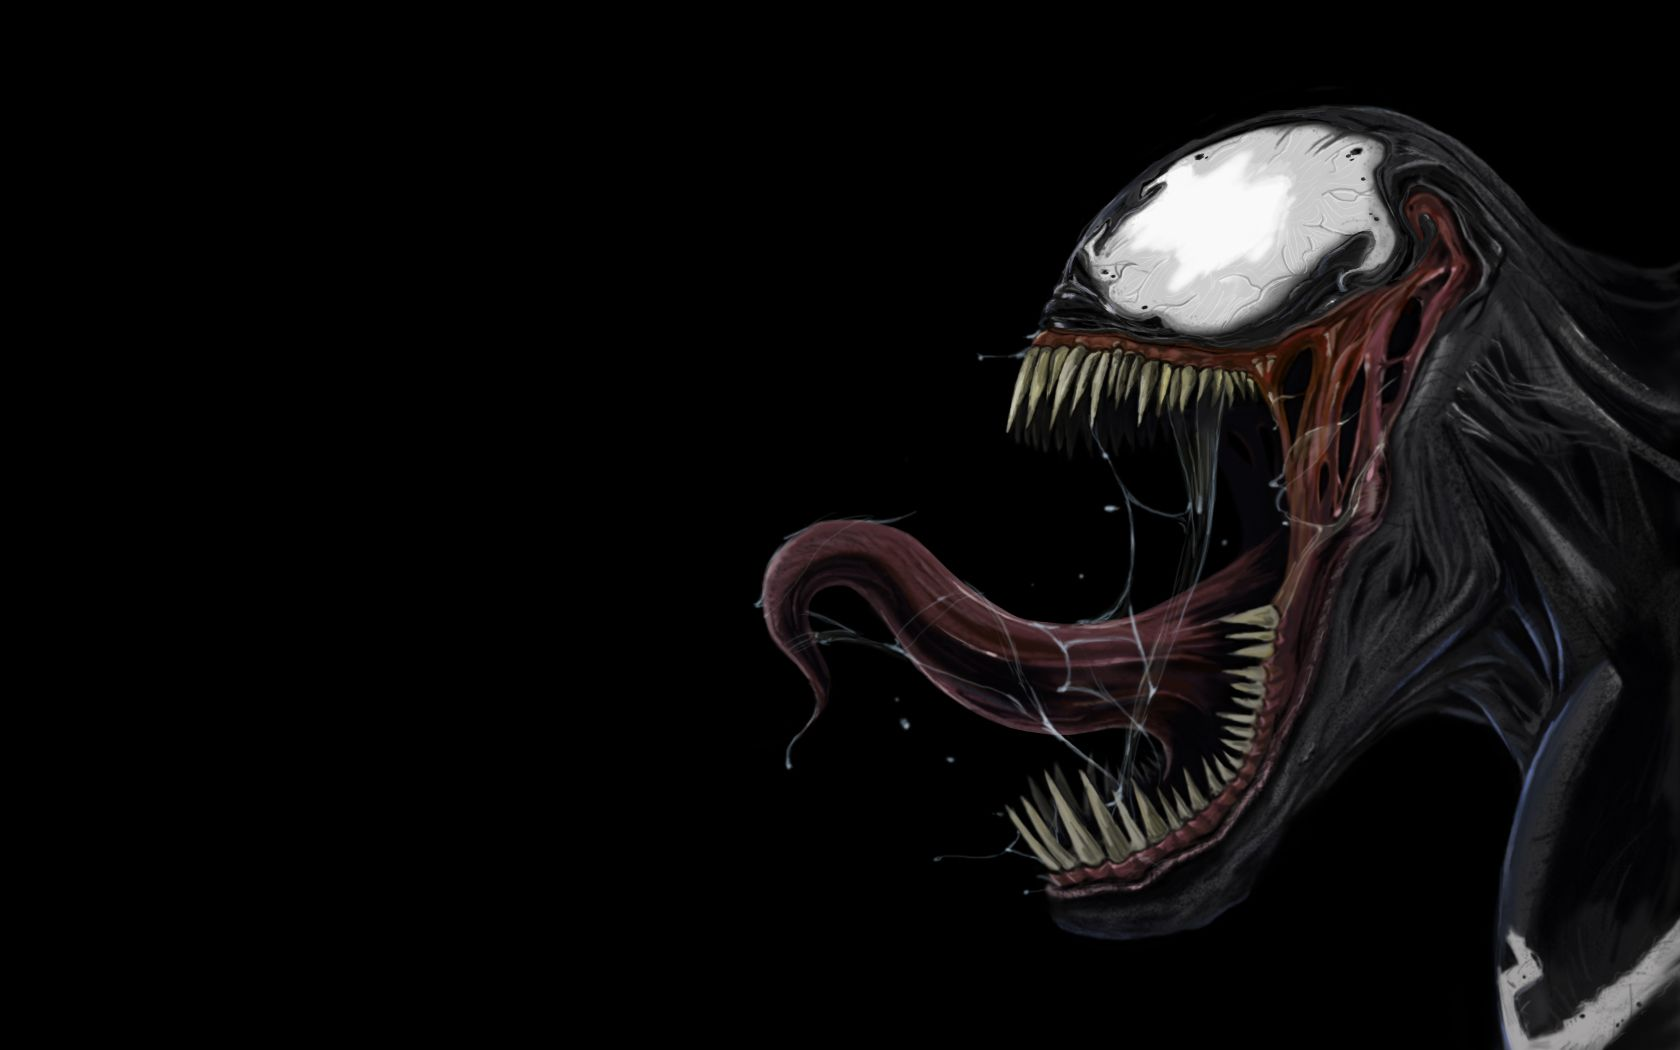
\includegraphics[width=\linewidth]{img.jpg}
    \caption{Image of venom}
    \label{fig:venom}
\end{figure}

\subsection{Multiple Images}

\begin{figure}[h!]
    \centering
    \begin{subfigure}[b]{0.4\linewidth}
        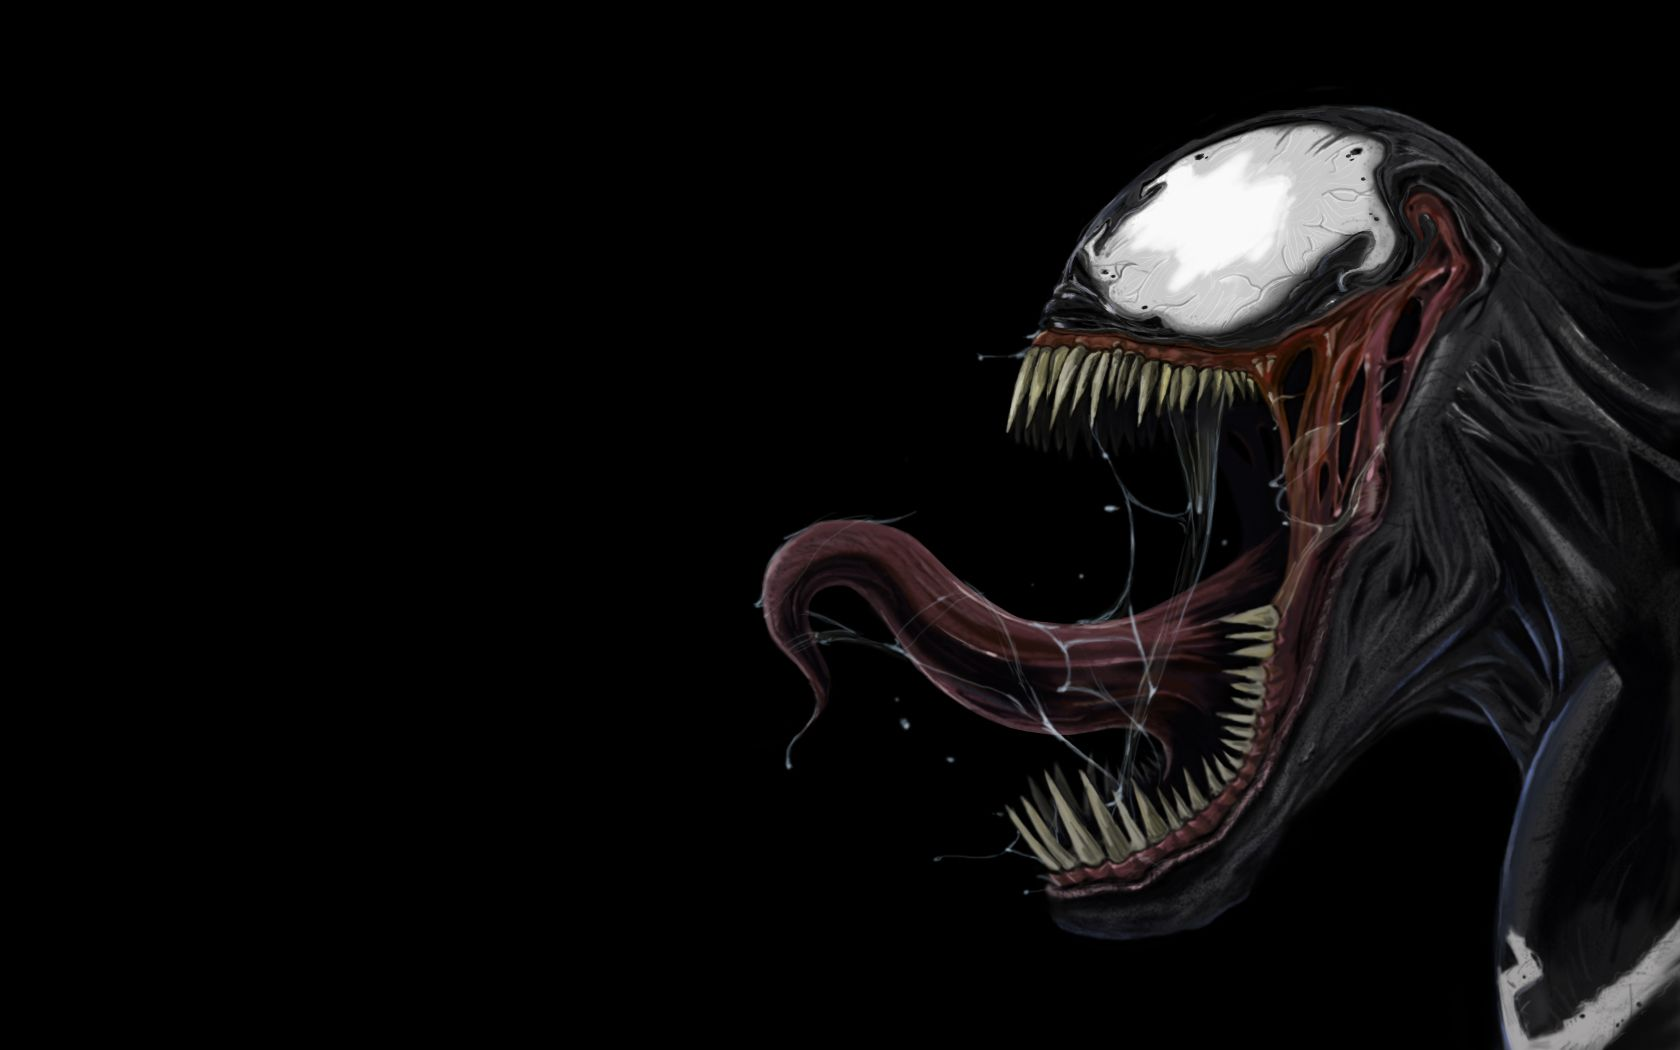
\includegraphics[width=\linewidth]{img.jpg}
        \caption{Venom.}
    \end{subfigure}
    \begin{subfigure}[b]{0.4\linewidth}
        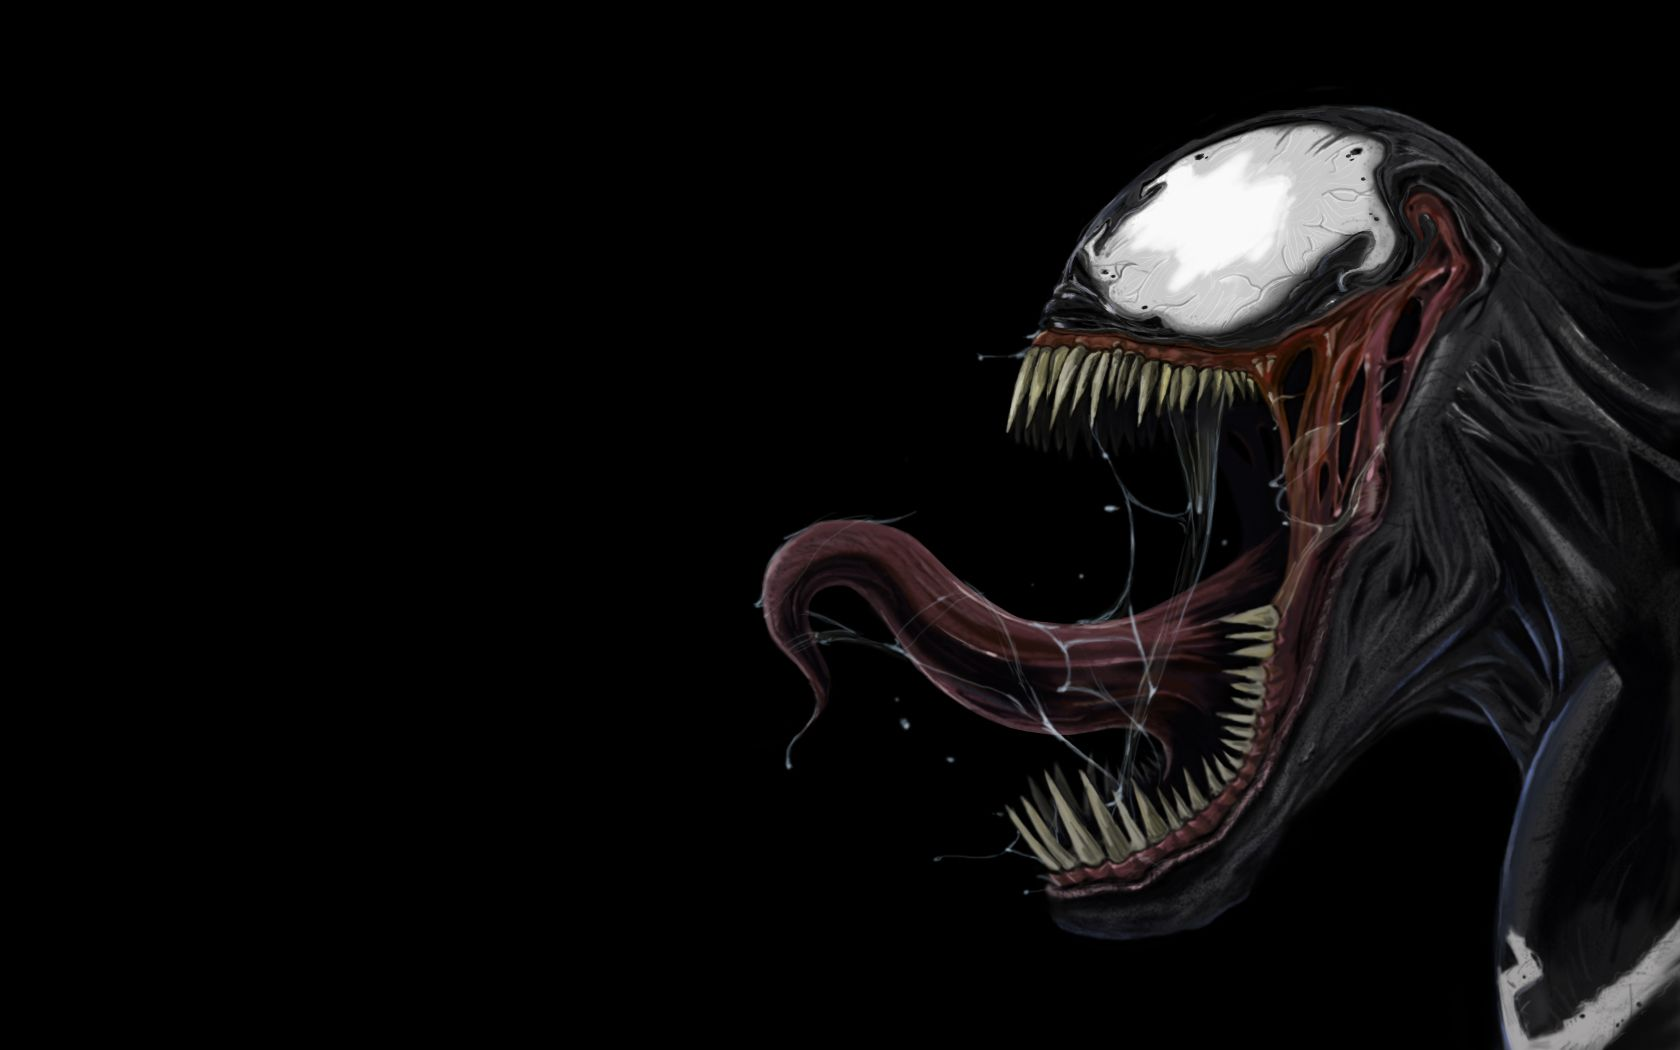
\includegraphics[width=\linewidth]{img.jpg}
        \caption{More Venom.}
    \end{subfigure}
    \caption{The same Venom. Two times.}
    \label{fig:coffee}
\end{figure}
\newpage
\subsection{More Position Formatting in Images}
\begin{figure}[h!]
    \centering
    \begin{subfigure}[b]{0.2\linewidth}
        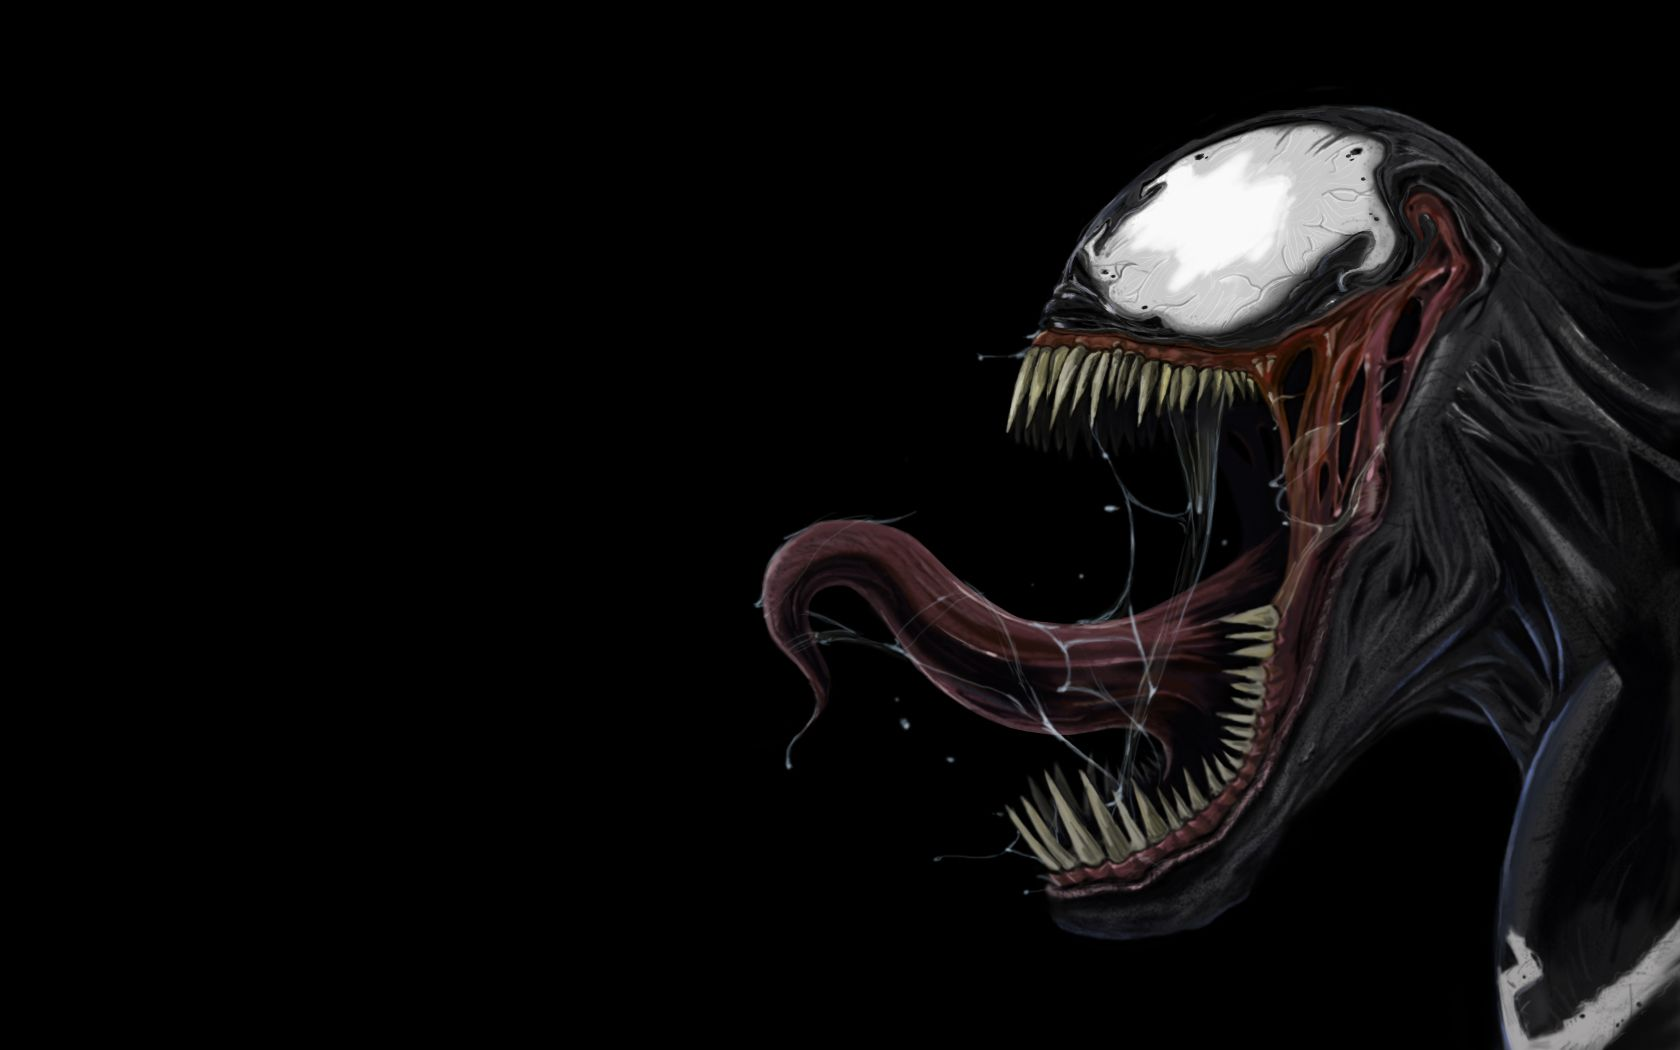
\includegraphics[width=\linewidth]{img.jpg}
        \caption{Venom}
    \end{subfigure}
    \begin{subfigure}[b]{0.2\linewidth}
        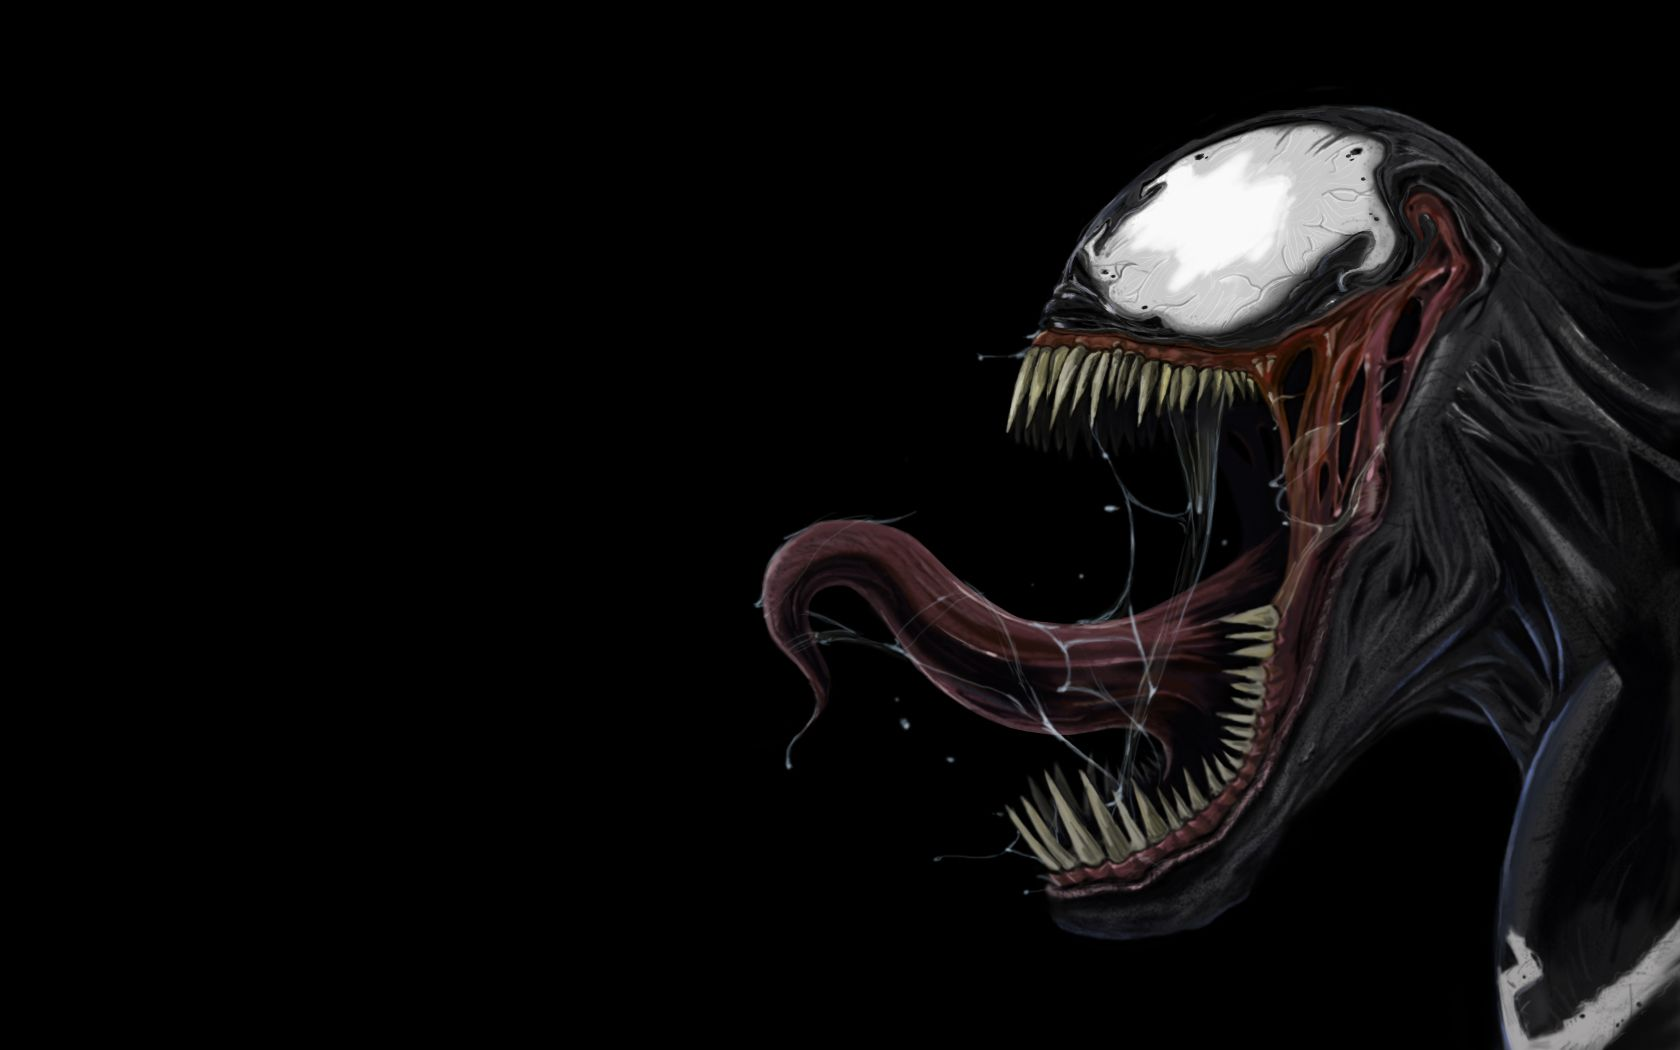
\includegraphics[width=\linewidth]{img.jpg}
        \caption{More Venom}
    \end{subfigure}
    \begin{subfigure}[b]{0.2\linewidth}
        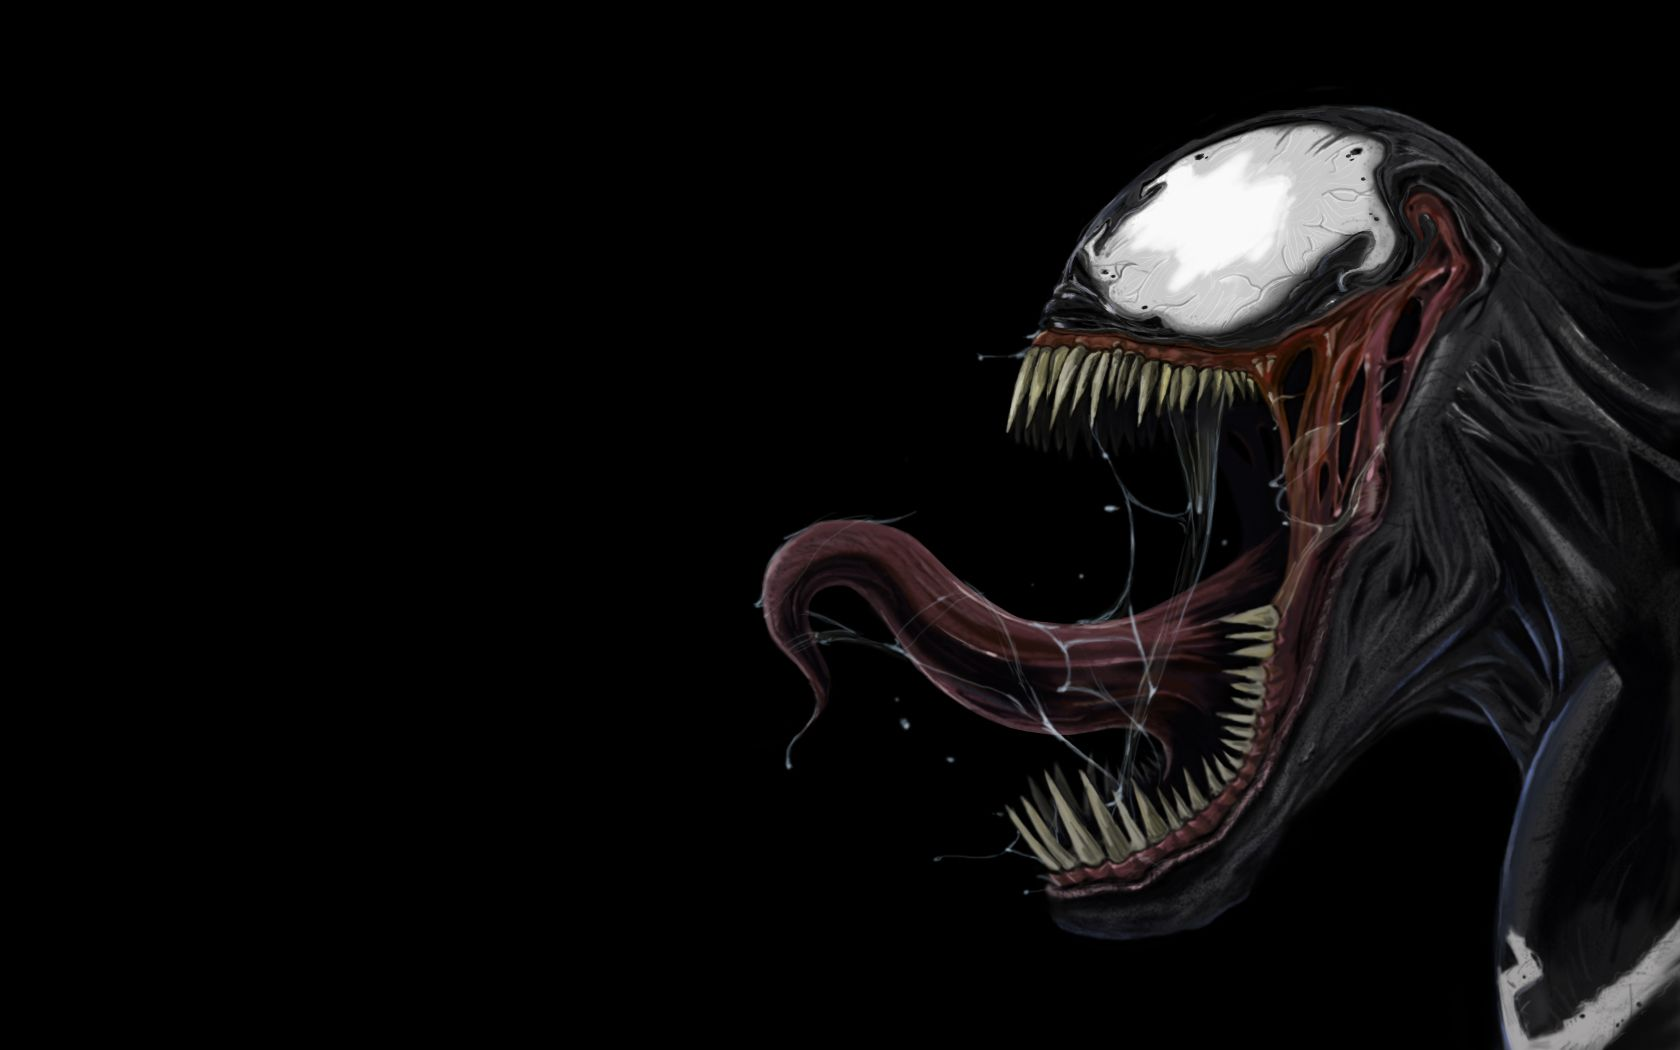
\includegraphics[width=\linewidth]{img.jpg}
        \caption{Danger}
    \end{subfigure}
    \begin{subfigure}[b]{0.5\linewidth}
        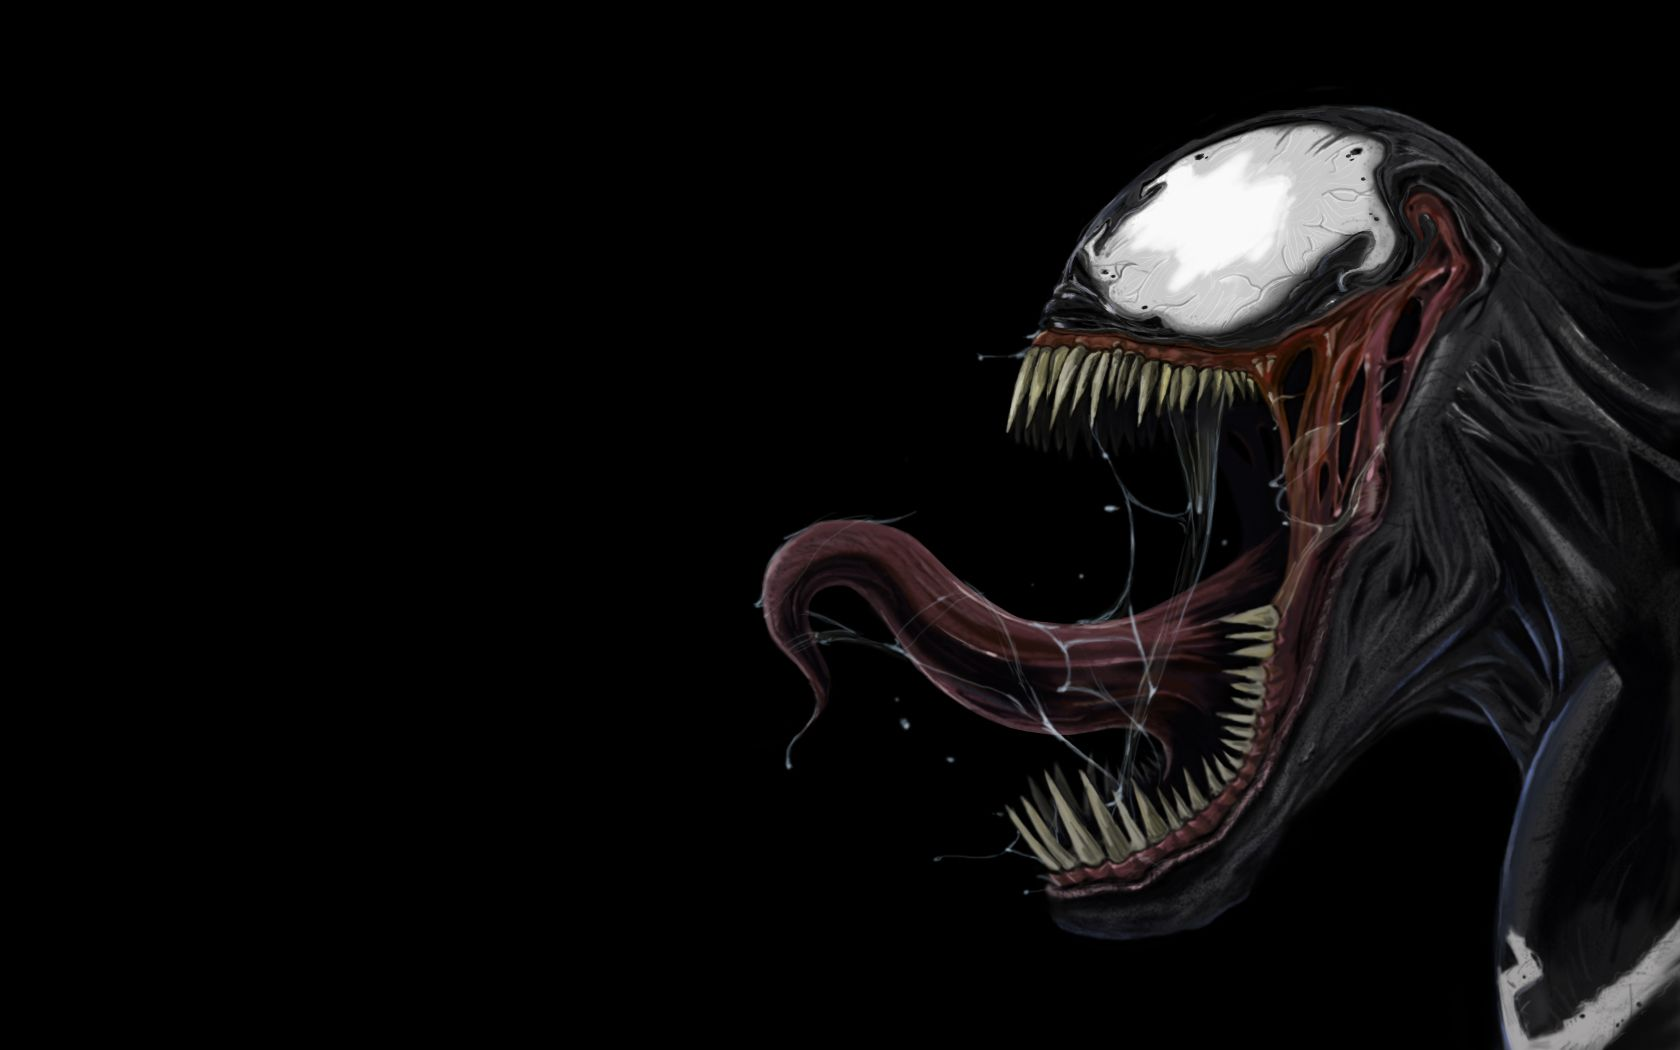
\includegraphics[width=\linewidth]{img.jpg}
        \caption{Too much Venom}
    \end{subfigure}
    \caption{Venom in Various Sizes}
    \label{fig:Different Size venoms}
\end{figure}

\section{Table Of Contents}
\subsection{Images and Tables in Table Of Contents}
Commented due to numbering problem
% \begin{appendix}
%     \listoffigures
%     \listoftables
% \end{appendix}

\section{Bibliography and Citations}
commented as doesn't works well with biblatex
% Random Citations \cite{einstein} embedded in text

\subsection{Footnote References}
Random Citations \autocite{gree00} embedded in text

\section{Footnotes}
This is some sample text \footnote{\label{myfootnote}Hello Footnote}\newline
I'm Referring to footnote \ref{myfootnote}.



\end{document}

